% Submission code: 8e3afa76-df76-4c8a-b6f4-cf5b8726e805
\documentclass{article}
\usepackage[utf8]{inputenc}
\usepackage{multicol}
\usepackage{listings}
\usepackage{amssymb}
\usepackage{enumitem}
\usepackage{graphicx}
\usepackage{amsthm}
\usepackage{hyperref}
\usepackage{tikz}
\usepackage[ruled, vlined]{algorithm2e}
\usepackage{mathtools}
\newtheorem{theorem}{Theorem}
\newtheorem{definition}{Definition}
\newcommand{\N}{\mathbb{N}}
\newcommand{\Np}{{\mathbb{N}^{>0}}}
\newcommand{\Z}{\mathbb{Z}}
\newcommand{\R}{\mathbb{R}}
\newcommand{\bigO}{\mathcal{O}}
\newcommand{\code}[1]{\texttt{#1}}
\newcommand{\hints}[1]{\paragraph{\bf Hints:} #1}

\SetKwProg{Fn}{Function}{}{}
\SetKwProg{Proc}{Procedure}{}{}
\SetKwFunction{hasEqualElementToIndex}{hasEqualElementToIndex}

\usetikzlibrary{arrows, positioning}

%=====================================
%			Assignment 8
%=====================================

\begin{document}

\title{Algorithms \& Datastructures \\ Weekly Assignment 9}
\date{\today}
\author{Tony Lopar \\ s1013792}
\maketitle
\section*{Exercise 1}
We start with an array of n elements, a possible way of a divide and conquer algorithm could be to split the array until we have pieces of one element. If we have this pieces of one element and we know the index of this element, we could check whether the values are equal.

At the beginning the array will be cut into two parts and for both parts there will be a recursive call. This continues until we have to check the arrays of one element. When one of the two recursive calls returns true, then we know that there is an equal index to an element and we should also return true. A possible implementation of this algorithm can be seen in algorithm~\ref{Alg:A1}.

The complexity of this algorithm is $O(log n)$, since the problem is split into two pieces every step.

\begin{algorithm}[ht!]
  \DontPrintSemicolon
  \Proc{\hasEqualElementToIndex{A, startI, endI}}{
  \If{$startI = endI$ and $A[starti] = startI$}{
    \KwRet{True} \;
  }
    $halfIndex \leftarrow startI + ((endI - startI) / 2)$ \;

    \If{\hasEqualElementToIndex{$A, startI, halfIndex$} or \hasEqualElementToIndex{$A, halfIndex, endI$}}{
      \KwRet{True} \;
    }
    \KwRet{False} \;
  }

    \caption{Algorithm that checks whether there is an $A[i] = i$} \label{Alg:A1}
\end{algorithm}

\newpage
\section*{Exercise 2}
\begin{enumerate}
  \item
  So we have to define the complexity of all the algorithms by induction.
  We will first start with Marieke which splits the problem into two of size $n-1$.
  So the formula for the complexity will be as follows.
  \begin{align*}
    T(n) =
    \begin{cases*}
        1, & \text{for n=1} \\
        2T(n - 1) + \bigO (n), & \text{for n $>$ 1}
    \end{cases*}
  \end{align*}
% \end{enumerate}

\paragraph{Marieke} When we calculate some values, we can find the closed formula for the algorithm of Marieke.
\begin{align*}
  T(1) &= 1 \\
  T(2) &= 2T(2 - 1) + c = 2T(1) + c = 2 + c \\
  T(3) &= 2T(3 - 1) + c = 2T(2) + c = 4 + 3c \\
  T(4) &= 2T(4 - 1) + c = 2T(3) + c = 8 + 7c \\
  T(n) &= 2T(n - 1) + c = 2T(2) + c = 2^{n-1} + (2^{n-1}-1)c
\end{align*}
In order to find the complexity we defined the formula $T(n) = 2^{n-1} + (2^{n-1}-1)c$. This formula should hold for all $n \geq 2$. We start at T(2), because T(1) has been defined specific as 1. \\
\textbf{Basis step} \\
We see that T(2) holds, because $2^{2-1} + (2^{2-1}-1)c = 2^{1} + (2^{1}-1)c = 2 + (2 - 1)c = 2 + c$ \\
\textbf{Inductive step} \\
  Let's assume that $T(k) = 2^{k-1} + (2^{k-1}-1)c$(IH) for all $k < n$. \\
  Now we have to prove that it also holds for $T(n)$. \\
  Hence we have to prove that $T(n) = 2^{n-1} + (2^{n-1}-1)c$
  \begin{align*}
    T(n) &= 2T(n - 1) + c \\
    &= 2(2^{n-2} + (2^{n-2}-1)c) + c \enspace (IH)\\
    &= 2 \cdot 2^{n-2} + 2 \cdot (2^{n-2}-1)c + c \\
    &= 2^{n-2+1} +  2(2^{n-2}-1)c + c \\
    &= 2^{n-2+1} +  (2^{n-2+1}-2)c + c \\
    &= 2^{n-1} +  2^{n-1}c -2c + c \\
    &= 2^{n-1} +  2^{n-1}c - c \\
    &= 2^{n-1} +  (2^{n-1}-1)c \\
    &\leq 2^n
  \end{align*}
  In terms of an asymptotic upperbound this shows us the formula that $T(n) \leq 2^n$.
This holds since the complexity of the algorithm is $O(2^{n-1} + (2^{n-1}-1)c)$ which is lower than $O(2^{n})$. The combining of the subproblems takes $O(n)$ which is smaller than the algorithm, so the complexity remains $O(2^{n})$.
\newline

\paragraph{Joost} The algorithm of Joost will have the complexity of:
\begin{align*}
  T(n) =
  \begin{cases*}
      1, & \text{for n=1} \\
      9T(\lceil n / 3 \rceil) + \bigO (n^2), & \text{for $n > 1$}
  \end{cases*}
\end{align*}

In order to make a guess for the asymptotic upperbound we will use the master theorem. Where we can fill in a = 9 and b = 3.
\begin{align*}
  T(n) &= aT(\frac{n}{b}) + f(n) \enspace \text{(Master theorem)}\\
   &= 9T(\frac{n}{3}) + \bigO (n^2) \\
   &= n^{log_3(9)} + \bigO (n^2) \\
   &= n^2 + \bigO (n^2)
\end{align*}

Knowing from the master theorem we see that $n^2$ equals the assymptotic upperbound. So from the master theorem we know that $T(n)$ has a complexity of $\bigO(n) = n^2 log n$.
\newline

\paragraph{David} The algorithm of David will have the complexity of:
\begin{align*}
  T(n) =
  \begin{cases*}
      1, & \text{for n=1} \\
      5T(\lceil n / 2 \rceil) + cn, & \text{for n $>$ 1}
  \end{cases*}
\end{align*}

In order to make a guess for the asymptotic upperbound we will use the master theorem. Where we can fill in a = 5 and b = 2.
\begin{align*}
  T(n) &= aT(\frac{n}{b}) + f(n) \enspace \text{(Master theorem)}\\
   &= 5T(\frac{n}{2}) + \bigO (n) \\
   &= n^{log_2(5)} + \bigO (n) \\
   &= n^{2.322} + \bigO (n)
\end{align*}

Knowing from the master theorem we see that $n^{log_2(5)}$ is higher the assymptotic upperbound of n. So from the master theorem we know that $T(n)$ has a complexity of ${\bigO (n^{\log _{2}(5)})}$.

\item The algorithm of Joost is the best, since the complexity of $\bigO (n^2 log n)$ is more efficient than the complexity of the other two algorithms.
\end{enumerate}

\newpage
\section*{Exercise 3}
In order to calculate the MAI we need to find the period where the total net income is higher than in any other period. We could define a divide-and-conquer algorithm by splitting up the array in half, so we have arrays with at most two elements. In these arrays we should calculate the sum of the two periods. If the sum has a positive result we should return both values of the period. If the sum is negative and one of the periods is positive we should only return this period. When a function gets two consecutive periods back from it's recursive calls, we should merge the periods. At the end we should check which period has the hightes MAI when there are multiple periods. Before this comparison at the end, we should remove any negative values at the start or end of the total periods. Since these can give a lower MAI than actual. After this we should iterate through the periods and return the one with the highest MAI.

The complexity of this algorithm can be computed using the master theorem. The combining will be in logaritmic time. For the combining we have to check whether the periods are consecutive. For this we only have to compare the periods from one call to the other period with the size of $log(n)$.

In order to make a guess for the asymptotic upperbound we will use the master theorem. Where we can fill in a = 2 and b = 2, since there are two recursive calls on half the list.
\begin{align*}
  T(n) &= aT(\frac{n}{b}) + f(n) \enspace \text{(Master theorem)}\\
   &= 2T(\frac{n}{2}) + \bigO (n) \\
   &= n^{log_2(2)} + \bigO (n) \\
   &= n^{1} + \bigO (n)
\end{align*}

\newpage
\section*{Exercise 4}
\emph{At the end of the description of the solution there is given an example for further clarification.}
\newline
In this situation we have a grid of $2^n \cdot 2^n$. This means that when the value of n increments with 1 we get a board of $2^{n+1} \cdot 2^{n+1}= 2^n \cdot 2 \cdot 2^n \cdot 2 = 4 \cdot 2^n \cdot 2^n$ which means the board will be 4 times bigger. This means that when we find a board for n which can be filled with tetrominos except for one cell, then when n increments we will have $4 \cdot 1 = 4$ cells that are empty. But in these 4 cells we can place a tetromino after which only one cell will remain empty.

A possible divide and conquer method could be to split the grid into 4 parts until we only have piece of $2 \cdot 2$ grids. In these grids we can place exactly one tetromino and have an empty cell. In the split we should give the position of the block in relation to the bigger grid to calculate how the tetromino should be placed. These positions can be rightupper(ru), rightlower(rl), leftupper(lu) and leftlower(ll). The tetromino should be placed in such a way that the cell in the grid with the opposite position of the grid stays empty. For example, a piece of the grid that is in the leftupper corner should have it's rightlower cell empty. When we combine the 4 smaller pieces, the 4 middle cells will be empty in this case. We can place one tetromino in these empty cells after which only one cell will be empty. In order to find out where this tetromino should be placed in the combined grid, we also should need where the grid of the combined pieces is in the total grid. If there's a bigger grid, then we should keep the cell that is in the grid most to the middle empty. We can keep this cell empty by rotating the inner grid with tetrominos by $180^\circ$. When the combined grid has the same size as the original we can keep the empty cell in the middle.

We can compute the complexity of this algorithm using the master theorem. In the combining we have to put a tetromino in, since we know the positions of the grid relative to the bigger grid we can instert this tetromino in constant time. Also the rotation of the inner grid is constant, since we already know the position in the grid. So, the complexity of the combining is $\bigO (1)$.

We can calculate the complexity of the algorithm using the master theorem. This will bring the complexity as follows:

\begin{align*}
  T(n) &= aT(\frac{n}{b}) + f(n) \enspace \text{(Master theorem)}\\
   &= 4T(\frac{n}{4}) + \bigO (1) \\
   &= n^{log_4(4)} + \bigO (1) \\
   &= n^1 + \bigO (1) \\
   &= n + \bigO (1)
\end{align*}

Knowing from the master theorem we see that $n^{log_4(4)}$ is higher the assymptotic upperbound of $\bigO (1)$. So from the master theorem we know that $T(n)$ has a complexity of $\bigO (n)$.

\subsection*{Example to clarify }
An example with of the algorithm with a grid of $2^2 \circ 2^2$ is shown below. In this example I will also show how we would modify this grid to combine it to a $8 x 8$ grid.

First, we start with a $2^2 x 2^2$ grid with all the 16 cells empty.   \\
\begin{center}
  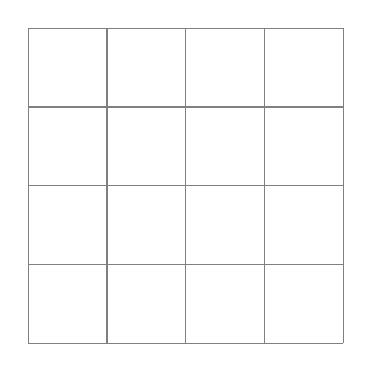
\begin{tikzpicture}
  \draw[step=0.5cm,color=gray, scale=2.0] (-1,-1) grid (1,1);
  \node[fill=white] at (-0.75,+0.75) {};
  \node[fill=white] at (-0.25,+0.75) {};
  \node[fill=white] at (+0.25,+0.75) {};
  \node[fill=white] at (+0.75,+0.75) {};
  \node[fill=white] at (-0.75,+0.25) {};
  \node[fill=white] at (-0.25,+0.25) {};
  \node[fill=white] at (+0.25,+0.25) {};
  \node[fill=white, scale=2.0] at (+0.50, 0.50) {};
  \node at (+0.75,-0.75) {};
  \end{tikzpicture}
\end{center}

We split this grid until we have multiple grids with 4 cells. And place a tetromino in such a way that the inner cell remains empty. The places tetrominos in the different pieces are marked with different colors. \emph{(The grid may be seen as 4 pieces of 2 x 2, but due to difficulty to realize this in \LaTeX\xspace it's shown as one grid)} \\
\begin{center}
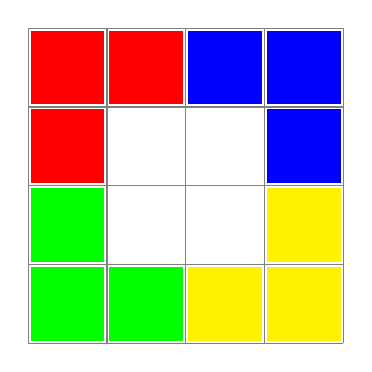
\begin{tikzpicture}
\draw[step=1cm,color=gray] (-2,-2) grid (2,2);
\node[fill=red, scale=4.0] at (-1.5,+1.5) {};
\node[fill=red, scale=4.0] at (-1.5,+0.5) {};
\node[fill=red, scale=4.0] at (-0.5,+1.5) {};
\node[fill=white, scale=4.0] at (-0.5,+0.5) {};

\node[fill=blue, scale=4.0] at (+0.5,+1.5) {};
\node[fill=white, scale=4.0] at (+0.5,+0.5) {};
\node[fill=blue, scale=4.0] at (+1.5, +1.5) {};
\node[fill=blue, scale=4.0] at (+1.5,+0.5) {};

\node[fill=green, scale=4.0] at (-1.5,-1.5) {};
\node[fill=green, scale=4.0] at (-1.5,-0.5) {};
\node[fill=green, scale=4.0] at (-0.5,-1.5) {};
\node[fill=white, scale=4.0] at (-0.5,-0.5) {};

\node[fill=yellow, scale=4.0] at (+0.5,-1.5) {};
\node[fill=white, scale=4.0] at (+0.5,-0.5) {};
\node[fill=yellow, scale=4.0] at (+1.5, -1.5) {};
\node[fill=yellow, scale=4.0] at (+1.5,-0.5) {};
\end{tikzpicture}
\end{center}

Now we have the 4 pieces filled with tetrominos, we can also place one tetromino in the empty cells in the middle. Assuming that this 4x4 grid is a leftupper piece of a bigger grid, we will place the tetromino in such a way the rightlower cell stays empty. \\
\begin{center}
  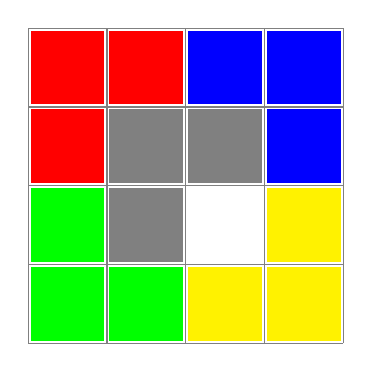
\begin{tikzpicture}
  \draw[step=1cm,color=gray] (-2,-2) grid (2,2);
  \node[fill=red, scale=4.0] at (-1.5,+1.5) {};
  \node[fill=red, scale=4.0] at (-1.5,+0.5) {};
  \node[fill=red, scale=4.0] at (-0.5,+1.5) {};
  \node[fill=gray, scale=4.0] at (-0.5,+0.5) {};

  \node[fill=blue, scale=4.0] at (+0.5,+1.5) {};
  \node[fill=gray, scale=4.0] at (+0.5,+0.5) {};
  \node[fill=blue, scale=4.0] at (+1.5, +1.5) {};
  \node[fill=blue, scale=4.0] at (+1.5,+0.5) {};

  \node[fill=green, scale=4.0] at (-1.5,-1.5) {};
  \node[fill=green, scale=4.0] at (-1.5,-0.5) {};
  \node[fill=green, scale=4.0] at (-0.5,-1.5) {};
  \node[fill=gray, scale=4.0] at (-0.5,-0.5) {};

  \node[fill=yellow, scale=4.0] at (+0.5,-1.5) {};
  \node[fill=white, scale=4.0] at (+0.5,-0.5) {};
  \node[fill=yellow, scale=4.0] at (+1.5, -1.5) {};
  \node[fill=yellow, scale=4.0] at (+1.5,-0.5) {};
  \end{tikzpicture}
\end{center}

Since in this example we assume that this grid is the leftupper piece of a bigger grid, we will rotate the rightlower piece $180^{\circ}$. This gives us the following grid. \\

\begin{center}
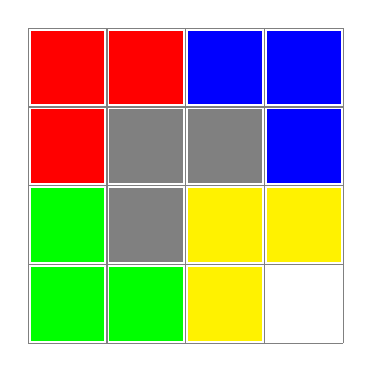
\begin{tikzpicture}
  \draw[step=1cm,color=gray] (-2,-2) grid (2,2);
  \node[fill=red, scale=4.0] at (-1.5,+1.5) {};
  \node[fill=red, scale=4.0] at (-1.5,+0.5) {};
  \node[fill=red, scale=4.0] at (-0.5,+1.5) {};
  \node[fill=gray, scale=4.0] at (-0.5,+0.5) {};

  \node[fill=blue, scale=4.0] at (+0.5,+1.5) {};
  \node[fill=gray, scale=4.0] at (+0.5,+0.5) {};
  \node[fill=blue, scale=4.0] at (+1.5, +1.5) {};
  \node[fill=blue, scale=4.0] at (+1.5,+0.5) {};

  \node[fill=green, scale=4.0] at (-1.5,-1.5) {};
  \node[fill=green, scale=4.0] at (-1.5,-0.5) {};
  \node[fill=green, scale=4.0] at (-0.5,-1.5) {};
  \node[fill=gray, scale=4.0] at (-0.5,-0.5) {};

  \node[fill=yellow, scale=4.0] at (+0.5,-1.5) {};
  \node[fill=yellow, scale=4.0] at (+0.5,-0.5) {};
  \node[fill=white, scale=4.0] at (+1.5, -1.5) {};
  \node[fill=yellow, scale=4.0] at (+1.5,-0.5) {};
  \end{tikzpicture}
\end{center}

If we combine this grid with the three other grids of the same size, the four middle cells will remain empty and we could agian put a tetromino in it and rotate a piece when necessary to have the grid covered with tetrominos.

\end{document}
